\documentclass[tikz,border=2pt]{standalone}
\usepackage{amsmath,amssymb}
\usepackage{xcolor}
\usetikzlibrary{positioning}
\begin{document}
% Extracted from namuenofull.inc; source column: \footnotesize \cite{NU}$_{\rm p{ 168 }}$ III$^*$-IV$^*$-$\alpha$
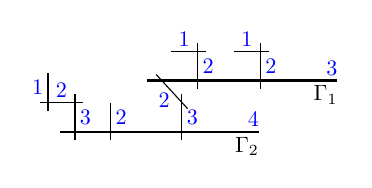
\begin{tikzpicture}[xscale=0.57,yscale=0.62]
\draw[thick,shorten >=2] (4/15,0)--(289/60,0) node[inner sep=2pt,blue,above left,scale=0.8] {4} node[inner sep=2pt,below left,scale=0.8] {$\Gamma_2$};
\draw[shorten <=-3pt, shorten >=-3pt] (3/5,0)--node[inner sep=2pt,scale=0.8,blue,right] {3} (3/5,3/5);
\draw[shorten <=-3pt, shorten >=-3pt] (3/5,3/5)--node[inner sep=2pt,scale=0.8,blue,above] {2} (0,3/5);
\draw[shorten <=-3pt] (0,3/5)--node[inner sep=2pt,scale=0.8,blue,left] {1} (0,6/5);
\draw[shorten <=-3pt] (7/5,0)--node[inner sep=2pt,scale=0.8,blue,right] {2} (7/5,3/5);
\draw[shorten <=-3pt, shorten >=-3pt] (179/60,0)--node[inner sep=2pt,scale=0.8,blue,right] {3} (179/60,3/5);
\draw[shorten <=-3pt, shorten >=-3pt] (179/60,3/5)--node[inner sep=2pt,scale=0.8,blue,below left=-1pt and -1pt] {2} (38/15,21/20);
\draw[thick,shorten >=2] (11/5,21/20)--(197/30,21/20) node[inner sep=2pt,blue,above left,scale=0.8] {3} node[inner sep=2pt,below left,scale=0.8] {$\Gamma_1$};
\draw[shorten <=-3pt, shorten >=-3pt] (10/3,21/20)--node[inner sep=2pt,scale=0.8,blue,right] {2} (10/3,33/20);
\draw[shorten <=-3pt] (10/3,33/20)--node[inner sep=2pt,scale=0.8,blue,above] {1} (41/15,33/20);
\draw[shorten <=-3pt, shorten >=-3pt] (71/15,21/20)--node[inner sep=2pt,scale=0.8,blue,right] {2} (71/15,33/20);
\draw[shorten <=-3pt] (71/15,33/20)--node[inner sep=2pt,scale=0.8,blue,above] {1} (62/15,33/20);
\end{tikzpicture}
\end{document}
